\documentclass[sigconf]{acmart}

\usepackage{graphicx}
\usepackage{hyperref}
\usepackage{todonotes}

\usepackage{endfloat}
\renewcommand{\efloatseparator}{\mbox{}} % no new page between figures

\usepackage{booktabs} % For formal tables

\settopmatter{printacmref=false} % Removes citation information below abstract
\renewcommand\footnotetextcopyrightpermission[1]{} % removes footnote with conference information in first column
\pagestyle{plain} % removes running headers

\newcommand{\TODO}[1]{\todo[inline]{#1}}

\begin{document}
\title{Big Data Analytics Using Regression Techniques}


\author{Nisha Chandwani}
\orcid{1234-5678-9012}
\affiliation{%
  \institution{Indiana University Bloomington}
  \city{Bloomington} 
  \state{Indiana} 
  \postcode{47405}
}
\email{nchandwa@iu.edu}

% The default list of authors is too long for headers}
\renewcommand{\shortauthors}{nchandwa}


\begin{abstract}
While analyzing large volumes of data, it is important to make sure that the data is analyzed accurately and efficiently for successful decision making. Predictive modeling has been one of the most critical aspects of analyzing big data. However, the traditional methods of predictive modeling cannot be directly applied to big data as applying statistical analysis to a large volume of data at once is a huge challenge in itself. We discuss how the traditional predictive methods, such as linear regression, can be modified for effectively modeling big data. We then discuss the distributed frameworks like Hadoop and Spark which help in predictive modeling of big data as well as the support extended by programming languages like R for these frameworks. Finally, we provide an overview of some of the regression techniques that can be applied for analyzing big data.
\end{abstract}

\keywords{i523, HID203, Big Data, Spark, Hadoop, Predictive Modeling, Regression}


\maketitle


\section{Introduction}

With increasing data from various sources, we have landed in the era of big data. However, collecting big data is just the first step. Effectively using this data for deriving useful business insights is of prime importance. Statistics is the art of learning from data for making optimal business decisions \cite{div-reg}. This learning from data involves the application of statistical methods like regression or time series modeling \cite{div-reg}. The present statistical techniques focus on deriving inference about the population based on sample data. Applying statistical methods to big data in one pass is a huge challenge and thus a more effective method is to partition big data into multiple samples. The results from all the samples can then be used to generate the final result for the predictive model. We present this method in detail in the following section and also discuss some of the regression techniques that can be effectively applied using this divide-and-conquer method on big data.

\section{Traditional Predictive Modeling}

Predictive modeling is one of the most important types of statistical analysis of big data. It aims to model the causal relationship between different features present in the data. Specifically, we try to predict the value of one variable, known as the dependent or response variable, with the help of one or more variables, known as independent or explanatory variables. The traditional predictive modeling process is shown in Figure \ref{fig:Fig1}.

\begin{figure}[!ht]
  \centering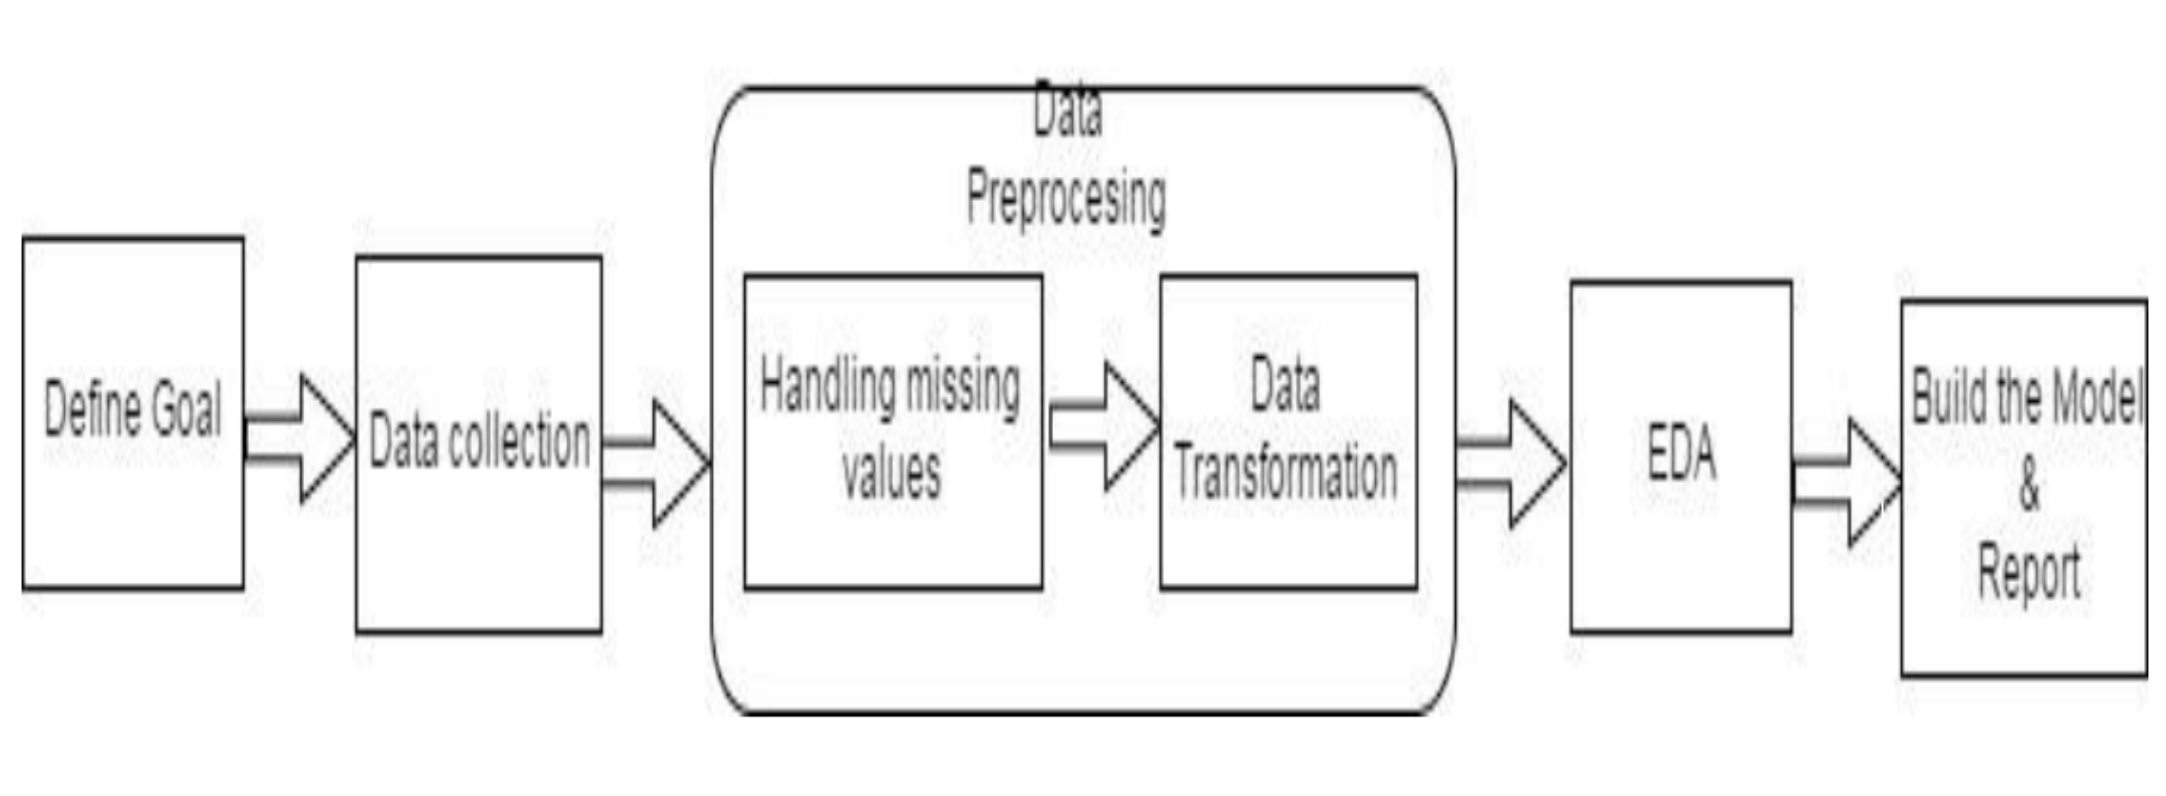
\includegraphics[width=\columnwidth]{images/Fig1.png}
  \caption{Steps in the predictive modeling process \cite{part-reg}}
  \label{fig:Fig1}
\end{figure}

Each of these steps in traditional predictive modeling is discussed in the following sections \cite{part-reg}.

\subsection{Define Goal}
For any predictive modeling, it is important to clearly define the goal, i.e., define the response variable and the explanatory variables that we are going to use to predict the response variable \cite{part-reg}.
\subsection{Data Collection and Management} 
This is another critical step for predictive modeling which requires identifying the data that can be used for analysis. It can be the most time-consuming step in the entire modeling process and may require some preliminary data exploration and visualization \cite{part-reg}. It also involves identifying the feature set and the structure of each feature.
\subsection{Data Preprocessing} 
Before building a predictive model, it is important to check the quality of data. Two major components of data preprocessing are \cite{part-reg}:
\begin{itemize}
	\item Analyzing missing values: For missing values, it is important to identify whether we want to drop the missing entries in the data or impute them using standard imputation methods such as mean imputation for quantitative features and mode imputation for qualitative features.
	\item Data transformation: The aim of data transformation is to convert it into a form which is easier to model. For example, normalization and standardization of data help in the better interpretation of the coefficients of the regression model. Some of the transformations also depend on the predictive model that we intend to apply. For example, for a linear regression model, it is important to ensure that the dependent and the independent variables have a linear relationship and that the dependent variable has a constant variance.
\end{itemize}
\subsection{Exploratory Data Analysis (EDA)} 
As part of EDA, we try to summarize the data graphically and analyze each feature along with the relationship between different features. For summarization, a variety of summary statistics such as mean, median, variance, etc. are used \cite{part-reg}. In case of predictive modeling, one might want to explore the data and visualize the numerical summary along with the correlation of different features in the data.
\subsection{Model-building and reporting}
The final step involves building the predictive model using the clean transformed data. Different regression techniques such as linear regression can be used for predicting the response variable from the independent variables. Basically, we try to estimate the coefficient, $\hat{\beta}$, for each independent variable such that a unit change in the independent variable results in a change of $\hat{\beta}$ units in the mean value of the response variable. Once the model is built, it is evaluated using one of the several metrics like the coefficient of determination.

\section{Predictive Modeling with Big Data}

After having the background of the traditional predictive modeling, we now study the process of extending this method for big data. Traditional statistical analysis generally rely on a representative sample of data to make inference about the population \cite{part-reg}. However, in case of big data, relying on one sample may lead to incorrect predictions. Thus, we partition big data into subsets such that the size of these subsets is close enough to a sample. We achieve this by using one of the sampling techniques from statistics such as random sampling, stratified sampling or cluster sampling \cite{div-reg}. We then apply regression techniques to each of these samples independently. The final prediction is made by aggregating the results from each of these samples. The architecture for this divide-and-conquer regression analysis is as shown in Figure \ref{fig:Fig2}. Except for the model building step, all other steps are the same as that of traditional predictive modeling.

\begin{figure}[!ht]
  \centering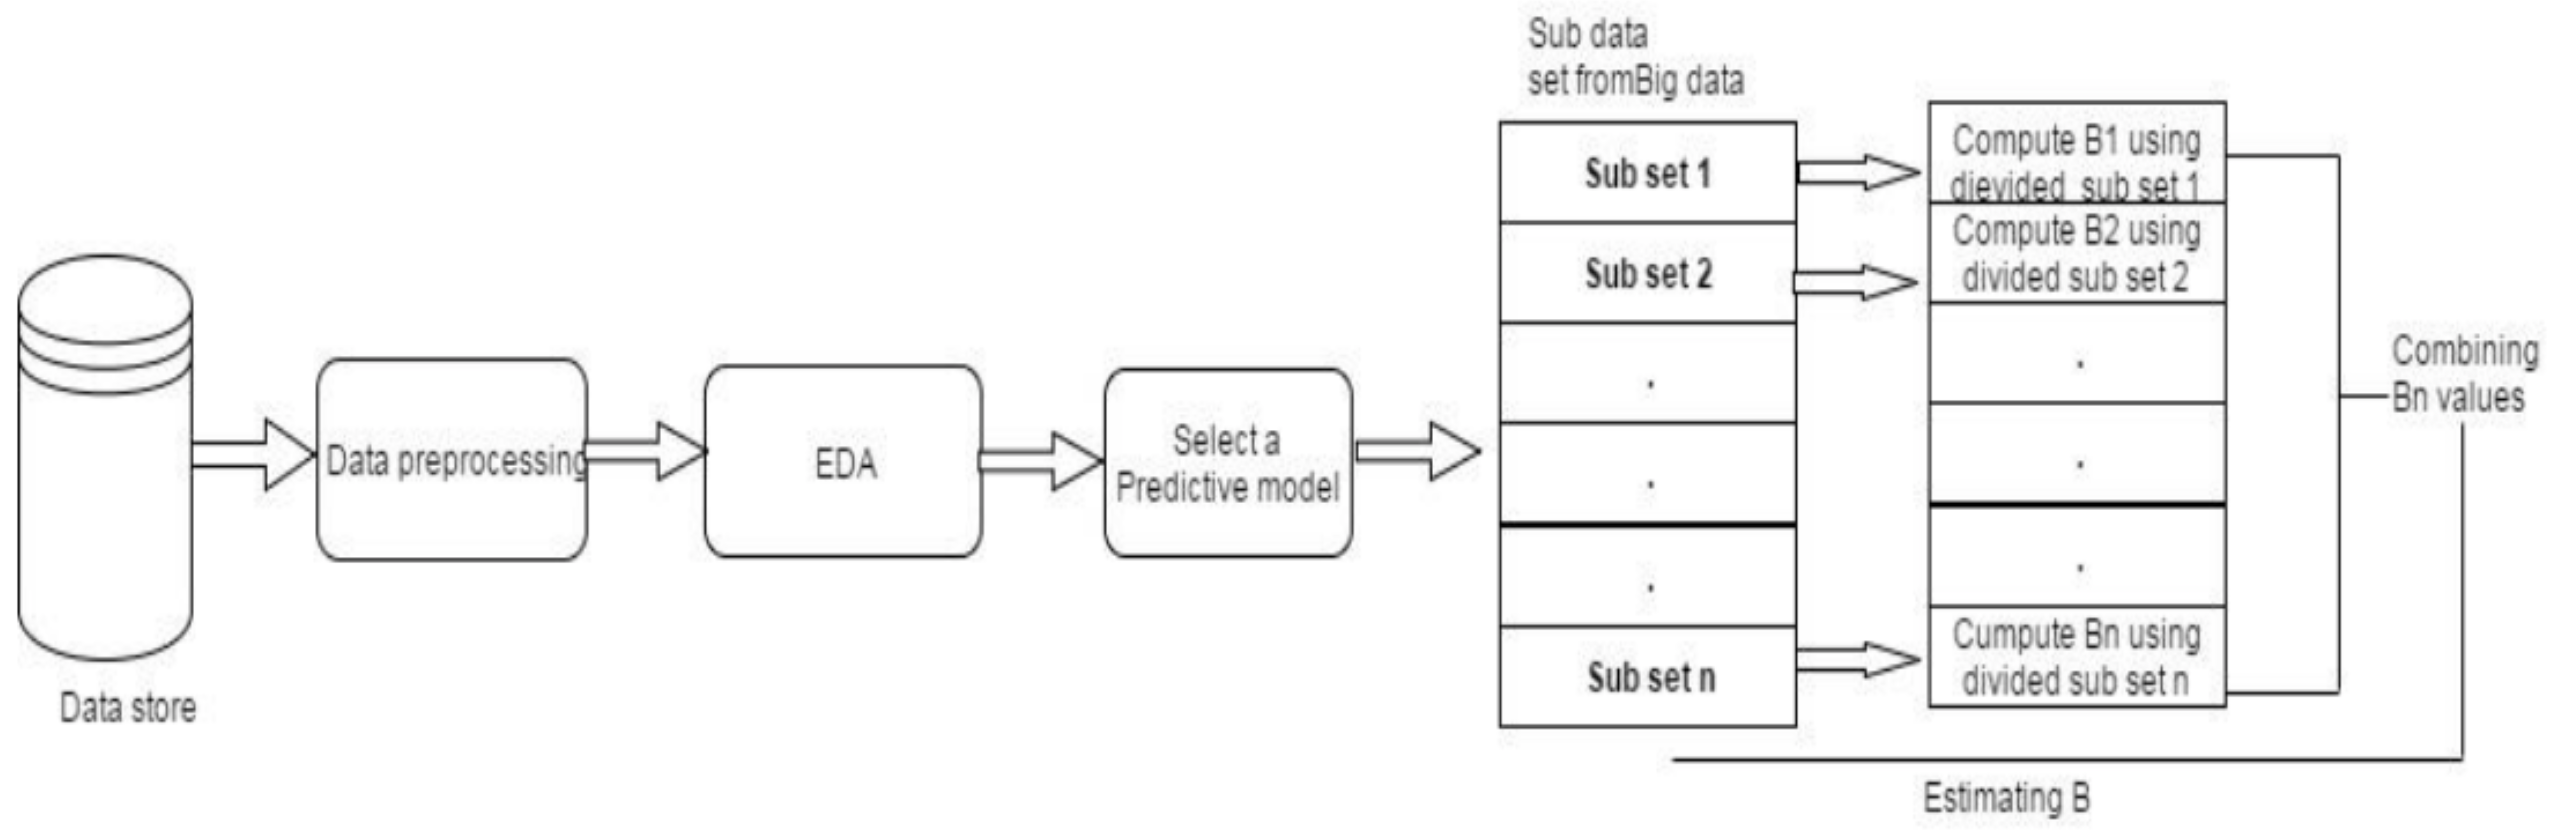
\includegraphics[width=\columnwidth]{images/Fig2.png}
  \caption{Architecture for partitioning Big Data \cite{part-reg}}
  \label{fig:Fig2}
\end{figure}

This divided regression analysis is summarized as below \cite{div-reg}:

\begin{itemize}
	\item Divide big data: In this step, the data is divided into $M$ subsets by using one of the statistical sampling techniques.
	\item Apply multiple linear regression analysis: Perform regression on each of these subsets and compute their respective regression parameters, $\hat{\beta_1}, \hat{\beta_2}, ...., \hat{\beta_m}$. Combine each of these parameters to compute the final regression co-efficient, $\hat{\beta_c}$ as below:
	\begin{center}$\hat{\beta_c} = f_c(\hat{\beta_1}, \hat{\beta_2}, ...., \hat{\beta_m})$\end{center}
	Here, $f_c$ is a combine function used for combining the co-efficients obtained from each of the $M$ subsets of data. This function can be defined in various ways based on the data. For example, we can define the combine function as the mean value of all the co-efficients: 
	\begin{center} $\hat{\beta_c} = \frac{1}{M}\sum_{i=1}^M \hat{\beta_i}$ \end{center}
	\item Evaluate the model: As part of model evaluation, we first check the confidence interval for all the co-efficients, obtained by applying the combine function, for all the independent variables. Next, we check the accuracy of the model by using some evaluation metric that measures how accurately the model predicts the value of the response variable. For example, we can use mean squared error ($MSE$) which is calculated as below:
	\begin{center} $MSE = \frac{1}{n}\sum_{i=1}^n (Y_i - \hat{Y_i})^2$ \end{center}
\end{itemize} 


\section{Big Data Systems and the support in R}
As explained in the previous section, regression analysis of big data can be efficiently performed by a divide-and-conquer strategy. However, it is important to remember that big data processing deals with a large volume of data and thus even in case of divided regression analysis, a single machine might not be enough. Thus, we require a distributed system where subsets of data are processed on multiple machines and the results are later aggregated to produce the final prediction as shown in Figure \ref{fig:Fig3} \cite{dkr-reg}.
\begin{figure}[!ht]
  \centering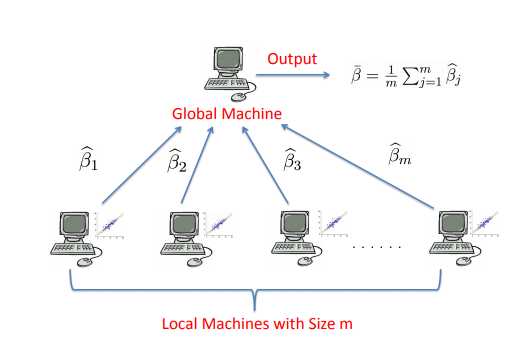
\includegraphics[width=\columnwidth]{images/Fig3.png}
  \caption{A divide-and-conquer learning framework \cite{dkr-reg}}
  \label{fig:Fig3}
\end{figure}
Some of the available frameworks that support such distributed storage and parallel computing include Hadoop and Spark. We can use the power of these frameworks to achieve the distributed version of traditional predictive modeling techniques. Many programming languages support these data-intensive computing paradigm. We discuss these frameworks and their support in one of the programming languages, i.e., R \cite{log-reg}.

\subsection{Hadoop} 
Hadoop is an open-source Java-based distributed computing platform which is used for distributed storage and distributed processing of huge data sets on computer clusters \cite{log-reg}. All the modules of the Hadoop framework are fault-tolerant, i.e., they can automatically handle failures of individual machines in the framework. The four important modules of this framework are \cite{log-reg}:

\begin{itemize}
    \item Hadoop Common provides all the Java libraries, utilities, OS level abstraction and the necessary files required by other modules
    \item Hadoop Distributed File System (HDFS) for storing big data as well as providing high throughput access to this data
    \item MapReduce for processing large volumes of data
    \item Hadoop YARN for resource management and task scheduling
\end{itemize}

R provides RHadoop, a family of R packages, that acts as a wrapper for Hadoop streaming and allows execution of Hadoop jobs \cite{log-reg}. Some of the important packages from RHadoop include rhdfs and rmr. Rhdfs is used for handling the HDFS operations such as file storage and file manipulation whereas rmr is primarily responsible for the map-reduce function \cite{log-reg}.

\subsection{Spark} 
Spark is another open-source distributed computing framework, however, unlike Hadoop, Spark is a memory based computing framework. Spark's in-memory processing capabilities often result in better performance as compared to Hadoop, especially when implementing iterative machine learning algorithms. The two key abstractions of Spark are:

\begin{itemize}
    \item Resilient Distributed Datasets: Collection of fault-tolerant data items which can be operated in parallel.
    \item Directed Acyclic Graph (DAG): DAG is a set of vertices and edges where vertices represent the RDDs and edges represent the operations to be applied to the vertices. Spark's DAG engine optimizes the execution by breaking down a Spark job into complex multi-step data pipeline to be executed on the cluster.
\end{itemize}

R provides the package SparkR which is a light-weight frontend for using Apache Spark in R \cite{log-reg}. SparkR provides SparkContext which establishes a connection between the R program and the Spark cluster. Users can then use the RDD class provided by this package to explore the Spark API and interactively trigger jobs from the R shell on to the Spark cluster. SparkR also provides distributed machine learning support through MLlib \cite{log-reg}. Thus, with the help of this package, we can implement a distributed version of the regression analysis.

\section{Regression Techniques for Big Data}

Using the distributed version, we can efficiently apply different kinds of regression for big data analysis. We now provide an overview of some of these regression techniques:

\subsection{Linear Regression}
Linear regression is one of the most widely used regression techniques. It tries to model the relationship between a dependent variable and one or more independent variables using a best-fit straight line which is represented by the equation below:
\begin{center} $y = \beta_0 + \beta_1 x$ \end{center}
The above gives the regression line, where $y$ represents the response variable and $x$ represents the independent variable, $\beta_0$ gives the intercept and $\beta_1$ gives the slope of the regression line. Once the coefficients, $\beta_0$ and $\beta_1$ are estimated, the regression line can be used to predict values of the response variable, $y$, for a given value of the explanatory variable, $x$. Linear regression has applications in various fields such as weather forecasting, stock price prediction, etc.

\subsection{Regularized Regression}
We always aim to build a machine learning model that generalizes well on the unseen data. Similarly, for regression, we would want to find the coefficients for the independent variables such that the resulting regression line has minimum prediction error for, not only the training data but also for the unseen test data. In order to prevent over-fitting in regression, we use regularized regression techniques such as ridge regression and lasso regression. Ridge imposes $L_2$ regularization whereas lasso imposes $L_1$ regularization on the coefficients of the independent variables. Ridge regression does a better job in presence of multicollinearity, i.e., when two or more independent features are correlated. Lasso regression does a better job when the number of independent variables is large. This is because the penalty imposed by lasso can shrink some of the coefficients to zero. Thus, lasso regression also provides feature selection in case of a large number of features.

\subsection{Logistic Regression}
Unlike linear regression which is used to predict the continuous value of the response variable, logistic regression is used when the response variable has a binary outcome. Thus, logistic regression is used for classification problems. It is used to model the relationship between the categorical response variable and one or more independent variables by estimating the probabilities using a logistic function \cite{log-reg}. Logistic regression has applications in many fields such as medical and social sciences \cite{log-reg}. For instance, it can be used to predict whether the patient is suffering from a given disease based on the various attributes related to the patient like age, sex, body mass index, blood levels, etc. Another application for logistic regression is predicting whether a candidate will vote Democratic or Republican based on his age, sex, race, social economic status.

\section{Conclusion}

While many companies are now focusing on accumulating big data, efficient analysis of this large volume of data is significant. We explained various stages of traditional predictive modeling and showed how it can be extended for big data. We also discussed the distributed frameworks like Hadoop and Spark that can be used for processing big data. These frameworks are supported by some of the programming languages such as R. With the help of these frameworks and the machine learning libraries supported by R, we can implement various regression techniques for building a predictive model for big data. Thus, by partitioning big data, we can effectively build prediction models which can be useful in various fields like medical, social sciences, etc.

\begin{acks}

  We would like to thank Dr. Gregor von Laszewski and the teaching assistants for their support and suggestions.

\end{acks}

\bibliographystyle{ACM-Reference-Format}
\bibliography{report} 


\end{document}
